%!TEX root = m392c_EHT_notes.tex
\begin{quote}\textit{
	``It's nice to write down, but oh so false.''
}\end{quote}
After defining a $G$-homotopy, the (well, a) natural question that might arise: what are $G$-weak equivalences and
$G$-CW complexes? This closely relates to obstruction theory: CW complexes are test objects.

To define $G$-CW complexes, we need cells. One choice is $G/H\times D^{n+1}$ and $G/H\times S^n$, where the actions
on $D^{n+1}$ and $S^n$ are trivial. This is a plausible choice (and in fact, will be the right choice), but it's
not clear why --- why not $G\times_H D(V)$ or $G\times_H S(V)$ for some $H$-representation $V$? Ultimately, this
comes from a (quite nontrivial) theorem that these can be triangulated in terms of the cells $G/H\times D^{n+1}$
and $G/H\times S^n$.\footnote{Illman's thesis~\cite{IllmanThesis} is a reference, albeit not the most accessible
one.} This is one of several triangulation results proven in the 1970s which are now assumed without comment, but
if you like this kind of math then it's a very interesting story.
\begin{defn}
A \term{$G$-CW complex} is a sequential colimit of spaces $X_n$, where $X_{n+1}$ is a pushout
\[\xymatrix{\coprod G/H\times S^n\ar[r]\ar[d] & X_n\ar[d]\\
\coprod G/H\times D^{n+1}\ar[r] & \pushout X_{n+1},
}\]
where $H$ varies over all closed subgroups of $G$.
\end{defn}
That is, it's formed by attaching cells just as usual, though now we have more cells.

This immediately tells you what the homotopy groups have to be: $[G/H\times S^n, X]$, which by an adjunction game
is isomorphic to $\pi_n(X^H)$. We let $\pi_n^H(X)\coloneqq \pi_n(X^H)$. Thus, we can define weak equivalences.
\begin{defn}
A map $f\colon X\to Y$ of $G$-spaces is a \term{weak equivalence} if for all subgroups $H\subset G$,
$f_*\colon\pi_n^H(X)\to\pi_n^H(Y)$ is an isomorphism.
\end{defn}
These homotopy groups have a more complicated algebraic structure: they're indexed by the lattice of subgroups of
$G$ and the integers. This is fine (you can do homological algebra), but some things get more complicated,
including asking what the analogue of connectedness is! (We'll broach this in \cref{equivariant_connected}.)

One quick question: do we need all subgroups $H$? What if we only want finite-index ones? The answer, in a very
precise sense, is that if you're willing to use fewer subgroups, you get fewer cells $G/H\times S^n$, and that's
fine, and you get a different kind of homotopy theory.

Finally, the Whitehead theorem (\cref{eqWhite}) is true for $G$-CW complexes. This follows for the same reason as
in May's course: it follows word-for-word after proving the equivariant HELP (homotopy extension lifting property)
lemma (\cref{HELP}) , which is true by the same argument as in the nonequivariant case.

$G$-CW complexes are just like the CW complexes we know and love, but with new cells $G/H$ indexed by the closed
subgroups $H\subset G$. The idea is that you're building up a space by attaching different spaces with different
isotropy groups ($G/H$ has isotropy group $H$, just by construction).
\begin{exm}[Zero-dimensional complexes]
The zero-dimensional complexes are $G/H$ or disjoint unions $\amalg_i G/H_i$. This is an instance of the slogan
that ``orbits are points.'' Keep in mind that if $G$ is a compact Lie group, this might not be zero-dimensional in
other, more familiar kinds of dimension.
\end{exm}
\begin{exm}
\label{S2sigmaCW}
Let $S^1$ act on $\R^2$ by rotation along the origin. This also induces a $C_n$-action, as $C_n\subseteq S^1$ as
the $n^{\text{th}}$ roots of unity. Let $V$ denote this $C_n$-space.

Let $D(V)$ denote the unit disc in $V$, and $S^V$ denote its one-point compactification, a representation sphere.
Then, $D(V)$ looks like wedges of pie, as the origin is fixed. On $S^V$, the point at infinity is also fixed, so we
obtain a beachball. % TODO picture

Now let's consider $V$ as an $S^1$-space, and write down the CW structure on $S^V$. There are two fixed points, and
each one is a $0$-cell $S^1/S^1\times *$, but there is one $1$-cell $S^1\times I$ attached to the endpoints
(thought of as a meridian rotated around the sphere).

Now let's consider the beachball for $C_2$ on $S^V$, where there are two hemispheres and $C_2$ rotates by a
half-turn. What's the $G$-CW structure on this?
\begin{itemize}
	\item There are two $0$-cells $C_2/C_2\times *$, corresponding to the two fixed points, the north and south
	poles.
	\item There is a single free $1$-cell $C_2\times I$, corresponding to the boundary of the hemispheres.
	\item There is a single $2$-cell $C_2\times D^2$.\qedhere
\end{itemize}
\end{exm}
Last time, we discussed other prospective cells $G\times_H S(V)$ and $G\times_H D(V)$; these can be decomposed in
terms of the actual cells we use.  One point to observe about these cells is that $G$ does not act on them by permuting non-equivariant cells around, but rather in a more complicated way; there is virtue in the simplicity of the $G$-cells we have chosen to work with.

\begin{ex}
$C_2$ also acts on $S^2$ by the antipodal map, which has no fixed points. Write a $C_2$-CW cell structure for this
$C_2$-space.
\end{ex}

\begin{exm}
\label{torusexm}
The torus $S^1 \times S^1$ has an $S^1$-action given by $z(z_1, z_2) = (zz_1, z_2)$. With this action, the torus
can be viewed as an $S^1$-CW complex with one $0$-cell $S^1/e \times *$ and one $1$-cell $S^1 \times [0,1]$, with
the attaching map sending $0$ and $1$ to $*$. Note that the largest cell we used here was a $1$-cell, whereas in
the nonequivariant construction of the torus, we are required to use a $2$-cell. Check out
\cref{equivariant_torus} for a picture.
\begin{figure}[h!]
\def\torlen{3}
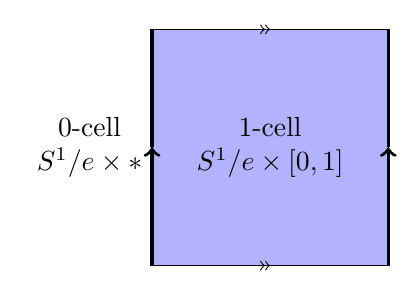
\begin{tikzpicture}[every node/.style={align=center}]
\draw[fill = blue!30!white] (0, 0) rectangle (\torlen, \torlen);
\draw[very thick, ->] (0, 0) -- (0, \torlen/2);
\draw[very thick] (0, \torlen/2) -- (0, \torlen);
\draw[very thick, ->] (\torlen, 0) -- (\torlen, \torlen/2);
\draw[very thick] (\torlen, \torlen/2) -- (\torlen, \torlen);
\draw[thin, ->>] (0, \torlen) -- (\torlen/2, \torlen);
\draw[thin] (\torlen/2, \torlen) -- (\torlen, \torlen);
\draw[thin, ->>] (0, 0) -- (\torlen/2, 0);
\draw[thin] (\torlen/2, 0) -- (\torlen, 0);
\node[left] at (0, \torlen/2) {$0$-cell\\$S^1/e\times *$};
\node at (1*\torlen/2, 1*\torlen/2) {$1$-cell\\$S^1/e\times[0,1]$};
\end{tikzpicture}
\caption{The $S^1$-CW structure on the torus in \cref{torusexm}. There is one $0$-cell and one $1$-cell.}
\label{equivariant_torus}
\end{figure}
\end{exm}
\begin{exm}
\label{triangle_exm}
Let $T$ be a solid equilateral triangle in the plane, so $D_6 = \ang{r,s\mid r^3 = s^2 = 1, srs = r^{-1}}$ acts on
it by rotations and reflections.
\begin{itemize}
	\item There are three $0$-cells: the center is a fixed point, so a $D_6/D_6\times *$. The three vertices are
	an orbit, with the stabilizer of each vertex conjugate to $\ang s$ inside $D_6$, so they form a $0$-cell of the
	form $D_6/\ang s\times *$. Similarly, the midpoints of each edge are an orbit with each stabilizer conjugate to
	$\ang s$, so they're also a $0$-cell of the form $D_6/\ang s\times *$.
	\item There are three $1$-cells: the three line segments from the center to a vertex are an orbit for $D_6/\ang
	s$, so form a $D_6/\ang s\times[0,1]$. Similarly, the three line segments from the center to the midpoint of an
	edge form a $D_6/\ang s\times[0,1]$. The six line segments from a vertex to the center of a midpoint are a free
	orbit of $D_6$, hence form a $D_6/e\times[0,1]$.
	\item The triangle minus these $0$- and $1$-cells is a free orbit, a $D_6/e\times D^2$.
\end{itemize}
See \cref{equilateral_triangle} for a picture.
\end{exm}
\begin{figure}[h!]
\tikzset{
    buffer/.style={
        draw,
        shape border rotate=90,
        isosceles triangle,
        isosceles triangle apex angle=60,
        fill=black!15!white,
        node distance=2cm,
        minimum height=4em,
		minimum width=5cm
    }
}
\def\TriangleLength{5}
\def\InscribedLength{0.288*\TriangleLength} % appx sqrt(3) / 6 times \TriangeLength
\begin{tikzpicture}
\node[buffer] {};
% 1-cells
\draw[line width=2pt, yellow!50!orange] (0, 0) -- (0, -\InscribedLength);
\draw[line width=2pt, yellow!50!orange] (0, 0) -- (-\TriangleLength/4, \InscribedLength/2);
\draw[line width=2pt, yellow!50!orange] (0, 0) -- (\TriangleLength/4, \InscribedLength/2);
\draw[line width=2pt, orange] (0, 0) -- (0, 2*\InscribedLength);
\draw[line width=2pt, orange] (0, 0) -- (-\TriangleLength/2, -\InscribedLength);
\draw[line width=2pt, orange] (0, 0) -- (\TriangleLength/2, -\InscribedLength);
\draw[line width=2pt, red] (-\TriangleLength/2, -\InscribedLength) -- (0, 2*\InscribedLength);
\draw[line width=2pt, red] (-\TriangleLength/2, -\InscribedLength) -- (\TriangleLength/2, -\InscribedLength);
\draw[line width=2pt, red] (\TriangleLength/2, -\InscribedLength) -- (0, 2*\InscribedLength);

% 0-cells
\draw[fill, blue] (-\TriangleLength/2, -\InscribedLength) circle (1mm);
\draw[fill, blue] (0, 2*\InscribedLength) circle (1mm);
\draw[fill, blue] (\TriangleLength/2, -\InscribedLength) circle (1mm);
\draw[fill, green!60!black] (0, 0) circle (1mm);
\draw[fill, purple!60!black] (0, -\InscribedLength) circle (1mm);
\draw[fill, purple!60!black] (-\TriangleLength/4, \InscribedLength/2) circle (1mm);
\draw[fill, purple!60!black] (\TriangleLength/4, \InscribedLength/2) circle (1mm);
\end{tikzpicture}
\caption{The $D_6$-equivariant structure on a solid triangle, as in \cref{triangle_exm}. Each cell is depicted in a
different color. The three $0$-cells are purple ($D_6/\ang s\times *$), blue ($D_6/\ang s\times *$), and green
($D_6/D_6\times *$); the three $1$-cells are yellow ($D_6/\ang s\times[0,1]$), orange ($D_6/\ang s\times[0,1]$),
and red ($D_6/e\times[0,1]$); the one $2$-cell is gray ($D_6/e\times D^2$).} \label{equilateral_triangle}
\end{figure}


There will be additional examples of $G$-CW complexes on the homework, some with richer structure.
\begin{rem}
At this point in class, the professor mentioned that these notes are hosted on Github at
\url{https://github.com/adebray/equivariant_homotopy_theory}. Since there aren't very many sources for learning
this material, and existing ones tend to have few examples, the hope is that these notes can be turned into a good
source of lecture notes for learning this material. So as you're learning this material, feel free to add
examples, insert comments (e.g.\ ``this section is confusing/unmotivated''), and let me know if you want access to
the repository.
\end{rem}
\begin{comp}{rem}{enumerate}
	\item There is a technical issue of a $G$-CW structure on a product of $G$-CW complexes; namely, there are
	technical difficulties in cleanly putting a $G$-CW structure on $G/H_1\times G/H_2$ involving triangulation.
	We won't digress into this: it's straightforward for finite groups, but a theorem for compact Lie groups, and
	required revisiting the foundations. Similarly, if $H\subset G$, we'd like the forgetful functor $G\Top\to
	H\Top$ to send $G$-CW complexes to $H$-CW complexes. This is again possible, yet involves technicalities.
	\item A nicer fact is that computing the fixed points of a $G$-CW complex is straightforward. Recall that
	$(\bl)^H$ is a right adjoint, which can be seen by realizing it as the limit of the diagram
	\[\xymatrix{
		\bullet\ar@(ur, ul)_H\ar[r] & \Top.
	}\]
	Thus, we don't expect it to commute with colimits in general. However, it does commute with many important
	ones, as in the following proposition.\qedhere
\end{comp}
\begin{prop}
The fixed point functor $(\bl)^H$ commutes with
\begin{enumerate}
	\item pushouts where one leg is a closed inclusion, and
	\item sequential colimits along closed inclusions.
\end{enumerate}
\end{prop}
This is great, because it means we can commute $(\bl)^H$ through the construction of a $G$-CW complex! In
particular, on each cell,
\[(G/K\times D^n)^H\cong (G/K)^H\times D^n,\]
so we need to understand $(G/K)^H\cong\Map^G(G/H,G/K)$. We will return to this important point.
\subsection*{Two approaches to the Whitehead theorem.}
We'll now discuss some homotopy theory of $G$-spaces and the Whitehead theorem. The first will be a hands-on proof
using the HELP lemma. This is an elegant approach to unstable homotopy theory due to Peter May in which one lemma
gives quick proofs of several theorems. In the equivariant case, it allows a quick reduction to the non-equivariant
case; it will be useful to see a proof of this nature. Ultimately, we will take a different approach involving
model categories, and this will be the second perspective.
\begin{defn}
Let $X,Y\in\Top$ and $f\colon X\to Y$ be continuous. Then, $f$ is \term{$n$-connected} if
$\pi_q(f)\colon\pi_q(X)\to\pi_q(Y)$ is an isomorphism when $q < n$ and surjective when $q = n$.
\end{defn}
We wish to generalize this to the equivariant case.
\begin{defn}
\label{equivariant_connected}
Let $\theta\colon\set{\text{conjugacy classes of subgroups of $G$}}\to\set{x\in\Z\mid x\ge -1}$.
\begin{itemize}
	\item A map $f\colon X\to Y$ of $G$-spaces is \term{$\theta$-connected} if for all $H\subset G$, $f^H$ is
	$\theta(H)$-connected.
	\item A $G$-CW complex is \term{$\theta$-dimensional} if all cells of orbit type $G/H$ have (nonequivariant)
	dimension at most $\theta(H)$.
\end{itemize}
\end{defn}
\begin{thm}[Equivariant HELP lemma]
\label{HELP}
Let $A$, $X$, $Y$, and $Z$ be $G$-CW complexes such that $A\subseteq X$ is $\theta$-dimensional and let $e\colon
Y\to Z$ be a $\theta$-connected $G$-map. Given $g\colon A\to Y$, $h\colon A\times I\to Z$, and $f\colon X\to Z$
such that $eg = hi_0$ and $fi = hi_1$, there exist maps $\tilde g\colon X\to Y$ and $\tilde h\colon X\times I\to Z$
that make the following diagram commute:
\[\xymatrix{
	A \ar[dd] \ar[rr]^-{i_0} && A\times I \ar[dd]|\hole \ar[dl]_-h && \ar[ll]_-{i_1} \ar[dl]_-g A \ar[dd]\\
	& Z && \ar[ll]_(0.35)e Y\\
	X \ar[ur]^-f \ar[rr]_-{i_0} && \ar@{-->}[ul]^-{\tilde h} X\times I && \ar[ll]^-{i_1} \ar@{-->}[ul]^-{\tilde g} X
}\]
\end{thm}
This is a massive elaboration of the idea of a Hurewicz cofibration. The best way to understand this is to prove
it (though it's not an easy proof).

In the non-equivariant case, one reduces to working one cell at a time, inductively extending over the cells of $X$
not in $A$.\footnote{This requires reducing to the case where $X$ is a finite CW complex, but taking a sequential
colimit recovers the theorem for all CW complexes $X$.} In this case, look at $S^{n-1}\subseteq D^n$. Now you just
do it: at this point, there's no way to avoid writing down explicit homotopies.
\begin{ex}
Think about this argument, and then read the proof in~\cite{ConciseCourse}.
\end{ex}
The equivariant case is very similar: in the same way, one can reduce to inductively attaching a single cell in the
case where $X$ is a finite CW complex. This comes via a map $G/H\times S^{n-1}\to G/H\times D^n$, but the only
interesting content is in the nonequivariant part, so we can reduce again to $S^{n-1}\to D^n$ with trivial
$G$-action! This allows us to finish the proof in the same way. It also says that the homotopy theory of $G$-spaces
is lifted from ordinary homotopy theory, in a sense that model categories will allow us to make precise.

The first consequence of \cref{HELP} is:
\begin{thm}
\label{estar}
Let $e\colon Y\to Z$ be a $\theta$-connected map and $e_*\colon [X,Y]\to [X,Z]$ be the map induced by composition.
\begin{itemize}
	\item If $X$ has dimension less than $\theta$, $e_*$ is a bijection.\footnote{We say that $X$ has dimension
	less than $\theta$ if for all closed subgroups $H\subset G$, all cells of orbit type $G/H$ have
	(nonequivariant) dimension at most $n$ for some $n \leq \theta(H)$.}
	\item If $X$ has dimension $\theta$, $e_*$ is a surjection.
\end{itemize}
\end{thm}
The proof is an exercise; filling in the details is a great way to get your hands on what the HELP lemma is
actually doing. Hint: consider the pairs $\emptyset\to X$ and $X\times S^0\to X\times I$, and apply the HELP lemma.
\begin{cor}[Equivariant Whitehead theorem]
\label{eqWhite}
Let $e\colon Y\to Z$ be a weak equivalence of $G$-CW complexes. Then, $e$ is a $G$-homotopy equivalence.
\end{cor}
\begin{proof}
This is also a standard argument: using \cref{estar}, $e_*$ is a bijection, so we can pull back
$\id_Z\in[Z,Z]$ to an inverse $(e_*)^{-1}(\id_Z)\in [Z,Y]$, which is a homotopy inverse to $e$.
\end{proof}
One can continue and prove the cellular approximation theorem in this way, and so forth. We won't do this, because
we'll approach it from a model-categorical perspective.

One thing that's useful, not so much for this class as for enriching your life, is to learn how to approach this
from the perspective of abstract homotopy theory, learning about disc complexes and so forth. You can prove
theorems such as the HELP lemma and its consequences in a general setting, and then specialize them to the cases
you need. This is a great way to ``just do it'' without needing model categories.

Anyways, we'll now define a model structure on $G\Top$ and $G\Top_*$. If you don't know what a model category is,
now is a good time to review.
\begin{prop}
There is a model structure on $G\Top$ (and on $G\Top_*$) defined by the following data.
\begin{description}
	\item[Cofibrations] The maps $f\colon X\to Y$ such that for all $H\subset G$, $f^H\colon X^H\to Y^H$ is a
	cofibration.
	\item[Weak equivalences] The maps $f\colon X\to Y$ such that for all $H\subset G$, $f^H\colon X^H\to Y^H$ is a
	weak equivalence.
\end{description}
\end{prop}
So we once again parametrize everything over subgroups of $G$ and use fixed points. This is a cofibrantly generated
model category; the cofibrations are specified by generators of acyclic cofibrations in a similar manner to $\Top$.
That is, in $\Top$, one can choose generators $I = \set{S^{n-1}\to D^n}$ and $J = \set{D^n\to D^n\times I}$; in
$G\Top$, we instead take $I_G = \set{G/H\times I}$ and $J_G = \set{G/H\times J}$.

These are cells that we used to define $G$-CW complexes, and this is no coincidence: it's a general fact about
cofibrantly generated model categories that follows from the small object argument\footnote{The small object
argument is a beautiful piece of basic mathematics that everybody should know. If you don't know it, your homework
is to read enough about model categories to get to that point. In general, there may be large objects and
transfinite induction, but for the case we care about large cardinals won't arise.} that cofibrant objects are
retracts of ``cell complexes'' built from the things in $I$, and cofibrations are retracts of cellular inclusions
of cell complexes. In this sense, CW complexes are inevitable.

The Whitehead theorem (\cref{eqWhite}) now falls out of the general theory of model categories.
\begin{thm}[Whitehead theorem for model categories]
Let $f\colon X\to Y$ be a weak equivalence of cofibrant-fibrant objects in a model category. Then, $f$ is a
homotopy equivalence.
\end{thm}
In $\Top$ and $G\Top$, all objects are fibrant, so this is particularly applicable.
